\section{Overview}
\begin{figure}[!ht]
\centering
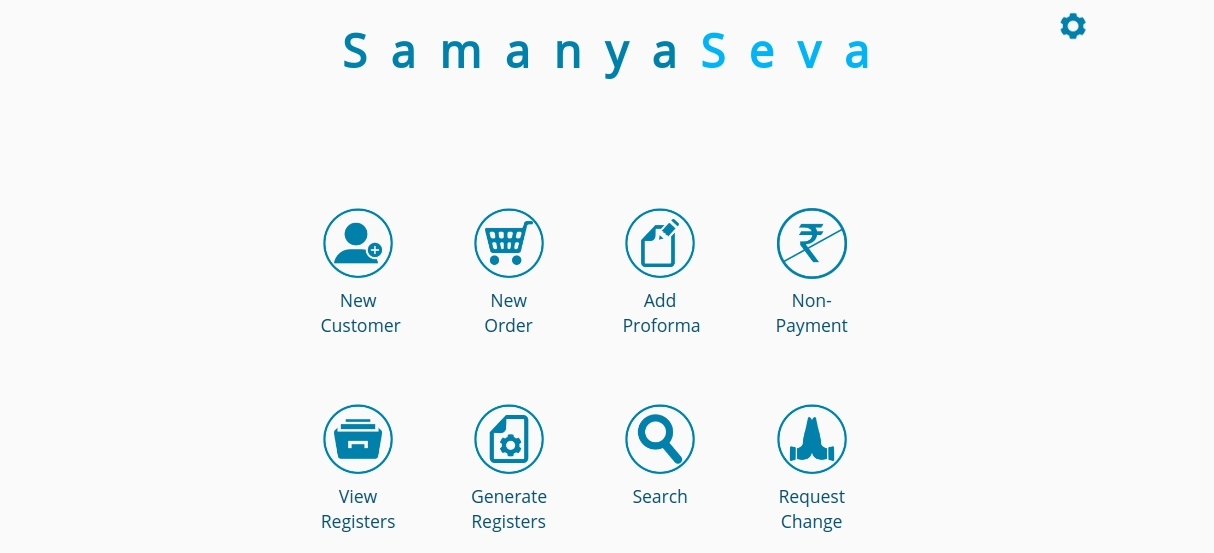
\includegraphics[scale=0.41]{input/images/samanya1.png}                   
\caption{Client Management Assure}
\hspace{-1.5em}
\end{figure}
\subsection{What is SamanyaSeva?}
 SamanyaSeva is an integrated software solution offered which can be used to support the seamless integration of information that flows through an organization. It is provided as a package comprising different modules, such as
Bills, Voucher, Catalog, Customer information etc.\\
It is basically an E-Commerce cum CRM (Customer relationship management) Django Web Application.
The basic idea behind it was to make a generalized E-commerce software that could be implemented in Companies as well as hospitals, bakery and other shops.\\\\
This project is basically a combination of people, processes and technology that seeks to understand a company's customers. It is an integrated approach to managing relationships by focusing on customer retention and relationship development.\\\\
CRM revolves around people, process and technology. SamanyaSeva has been developed using the latest technologies. 


\section{The Existing System}
There are few existing systems which do the task like Busy, SAP or other softwares but
they don't have few features which are here in this system. These system were not open source
and free web based software.
All exiting system suffers from at least one of the following system.
 \subsection{Limitations of previous system }
\begin{itemize}
\item No Modular Approach. 

\item No Independent modules such as Catalog.

\item Can't be easily configured for different purposes.


\end{itemize}
\section{Technologies Used}
\begin{enumerate}
\item Web Development languages (JS, HTML, CSS)
\item Django (Python Framework)
\item Bootstrap
\item MySQL
\item Apache
\item Hovercraft
\item LaTeX
\item Git

\end{enumerate}

\section{Objective of Project}
SamanyaSeva is a CRM cum ERP Application and the 
main objectives of this project is to :
\begin{enumerate}
\item Enhancing the operational efficiency of business resources. 
\item To make an open source project in which people can contribute and learn.
\item To follow modular approach for easy configuration.
\end{enumerate}


\newpage


